\documentclass{article}

\usepackage{amsmath, amsfonts, array, authblk, float, graphicx, hyperref, natbib, subcaption}
\usepackage[margin=1in]{geometry}

\bibliographystyle{../apa-good}
\linespread{1.2}

\title{A comps-based approach for interpreting tree-based predictions with an application to the NFL draft}
\author[1]{Elisabeth Millington}
\author[2]{Scott Powers}
\affil[1]{Department of Kinesiology, Rice University}
\affil[2]{Department of Sport Management, Rice University}

\begin{document}

\maketitle

\begin{abstract}
  Random forests are a powerful yet opaque machine learning predictive model. This poses challenges for interpretability, particularly in environments where decisions can be very high-stakes, like professional sports. In this paper, we present a method for interpreting random forest predictions in a sports setting through the lens of player comps. Player comps are a common practice in player scouting, where prospects are evaluated based on their perceived similarity to past players. We can define interpretable similarity scores that quantify how much each training observation contributes to a given prediction by leveraging the connection between random forests and adaptive nearest neighbors. A player’s similarity scores can be viewed as quantifiable player comps. We apply this methodology to evaluate quarterback prospects in the 2025 National Football League Draft using ESPN’s Total Quarterback Rating (QBR) per season, which has been regressed to zero based on attempts per season as the outcome variable. We show that our approach captures meaningful structure in the data while providing interpretability, allowing us to identify comps for top prospects such as Cam Ward, Jaxson Dart, Shedeur Sanders, and Dillon Gabriel.
\end{abstract}

\section{Introduction}

Random forests are a powerful machine learning prediction model that use the ensemble learning technique of combining multiple decision trees to mitigate overfitting. Each tree is built from a random bootstrap of the data, and the final prediction is determined by either majority tree vote (classification tasks) or averaging the tree responses (regression tasks). Random forests have the flexibility to model many different functional relationships while maintaining robustness to noise and outliers within the data \citep{breiman_random_2001}, which makes them suitable for many real-world applications.

Like other so-called ``black box'' machine learning algorithms, one drawback of the random forest is that the reasons for an individual's prediction can be difficult to interpret. Interpretability is crucial when using a machine learning algorithm because it allows the user to choose the best prediction method and it builds trust for the user in the prediction \citep{ribeiro_why_2016}. This is especially important in sports contexts because executives need to consider non-quantifiable information in their decision-making. The better a user understands how a model arrives at a prediction, the better they can determine how much it is appropriate to adjust the prediction based on subjective information from outside of the model.

Perhaps one of the most important decisions that sports executives make is selecting quarterbacks in the National Football League (NFL) draft. Quarterbacks are the backbone of offensive schemes for every NFL team and are arguably the most important position \citep{hughes_positional_2015}. Due to the nature of the position, trading for or signing a solid quarterback during free agency is uncommon, which is why drafting a quarterback with high NFL potential is crucial for team success. Since quarterbacks are highly sought after, talented college quarterbacks with perceived NFL starting potential are typically taken in the first or second round of the draft. In the NFL, this can have significant consequences because the rookie salary scale means large financial commitments to players taken at the top of the draft. In 2025, the slotted contract for No. 1 pick Cam Ward was \$48.4 million over four years, of which \$32.2 million was guaranteed as signing bonus \citep{badenhausen_nfl_2025}.

In traditional scouting for sports, draft prospect discussions and predictions are often based on comparing a current prospect with similar draft prospects in the past. Some of these past draft prospects will have gone on to successful careers, and others will have experienced less success \citep{trapasso_nfl_2025}. Scouts, managers, and coaches can assess NFL potential by comparing prospects to past players with similar collegiate careers. These historical reference players are known colloquially as ``comps'' \citep{jones_nfl_2025}, short for comparables. The simplest example of this line of reasoning is, ``This prospect reminds me most of Player X, and Player X had a successful career, so I think this player will have a successful career,'' effectively a human implementation of the $k$-nearest neighbor ($k$-NN) algorithm, with $k = 1$.

Random forests can be thought of as an adaptive $k$-NN algorithm \citep{lin_random_2006}, with the nearness of neighbors adaptively determined to minimize prediction error. Our work is moivated by this connection between random forests and the traditional lens of player comps. In this paper, we develop methods and software for extracting similarity scores from fitted random forest models in such a way that the prediction for a new data point is the weighted average of the outcomes in the training set, weighted according to these similarity scores.

The paper is organized as follows. In Section \ref{sec:data}, we describe a dataset on which we apply our methodology to evaluate NFL draft quarterback prospects, using ESPN's Total Quarterback Rating as the response variable and college statistics as the predictor variables. In Section \ref{sec:methods}, we derive similarity scores from a fitted random forest such that the model's predictions are equal to a similarity-weighted average of the training outcomes. In Section \ref{sec:results}, we interpret the predictions from the NFL quarterback draft prospect random forest model by ranking players from the training set according to their similarity scores induced by the adaptive nearest neighbors interpretation of random forests. In Section \ref{sec:software}, we describe the new R package rfcomp for calculating these similarity scores from fitted random forest objects. In Section \ref{sec:discussion}, we summarize the key findings.

\subsection{Related Work}

Previous research has been done to attempt to introduce interpretability to predictions from random forests and other tree-based machine learning algorithms. \citet{petkovic_improving_2018} describe a user-centered approach to reporting random forest results in an interpretable manner. \citet{aria_comparison_2021} compare two different techniques for interpreting the interactions between predictor variables and response variables in random forest models. In a sports context, \citet{ouyang_integration_2024} use Shapley Additive exPlanations (SHAP) values to interpret NBA game outcome predictions from an XGBoost model.

Draft models are fairly common in professional sports, as evaluating prospect talent can be key to success. One example of a draft model that uses ESPN's Total Quarterback Rating as the response variable is \citet{craig_predicting_2021}. They used logistic regression to estimate whether a quarterback would be selected in the draft and used a second regression to estimate that quarterback's NFL performance based on their final season metrics, scout grades, and player height. Their predictions are easy to interpret directly from the logistic regression model. \citet{wolfson_quarterback_2011} use their own metric of net points combined with games played to define NFL success. They estimate a logistic regression model for this metric on a combination of NFL Combine and college statistics, and they use this model to analyze how effectively NFL teams leverage data available when drafting a quarterback. Again, the logistic regression model results in predictions that are easily interpretable. \citet{berger_jumping_2021} use principal component analysis (PCA) combined with a high-order regression model to evaluate NBA prospects using their college statistics and combine data. The interpretation of the principal components is unclear, resulting in a relatively uninterpretable draft model. \citet{luo_improving_2024} propose a method for improving the way that NHL teams draft players by using both scouting reports and statistics. They use a combination of large language models and ensemble machine learning, which are both opaque in the way that they generate predictions, leading to uninterpretable predictions/reports.

While past work in sport analytics has attempted to predict draft prospect outcomes using interpretable methods (i.e. logistic regression) or machine learning methods with greater predictive accuracy, the novelty of the current work is that we achieve interpretability with a machine learning moethod. In particular, we tie our novel interpretation of random forest predictions to the concept of comps, which is well understood by scouts and executives in the sports industry. The implementation of our method is available in the treecomp R package, allowing practitioners to easily apply it to their own fitted random forests.

\section{Data}
\label{sec:data}

All data used for this study are publicly available from Sports Reference \citep{sports_reference_sports_2025}. Our dataset includes 2,114 quarterbacks who played their final season at the NCAA Division I Football Bowl Subdivision (FBS) between 2001 and 2023 (inclusive) who played more than six total games in their careers and attempted more than five passes per season. The data for each player-season include team, conference, strength of schedule, games played, passing statistics (attempts, completions, touchdowns, interceptions), rushing statistics (attempts, yards, touchdowns), and awards (All-America designation, Heisman voting).

In addition to college statistics, we obtained each player's passing attempts and Total Quarterback Rating (QBR) \citep{burke_how_2016} from each season between 2006 and 2024 (inclusive). Only available since 2006, QBR is based on expected points added (EPA), which is the change in drive scoring expectation before and after each play. It considers each quarterback's share of their team's EPA and accounts for home-field advantage, defensive strength, and garbage time. The range of QBR is from 0 to 100, and \citet{burke_how_2016} suggests thinking of it as a percentile of performance at the individual game level. For each quarterback, we calculate their average QBR per season, and we define a player who has attempted fewer than 10 career NFL passes to have a QBR of zero. Here the scale of QBR is helpful because players who reach the NFL cannot be rated below players who never reach the NFL. 

Since it is possible for a quarterback with very few pass attempts to have a high QBR, we adjusted the average QBR by regressing it toward zero based on attempts per season. We used attempts per season rather than career attempts to prevent discrimination against players who have not yet played many seasons. We used the formula $QBR_{adj}=/frac{avg_att*\bar{QBR}}{avg_att+c}$ for regression, where c is a constant. We used a nonlinear least squares model with a formula of $QBR2~/frac{(Att * QBR)}{(Att + c)}$, where Att is that season's total attempts, QBR is that season's QBR, and QBR2 is the next season's QBR, to find c, resulting in a value of 22.50. 

Average QBR per season is the response variable describing the success of quarterback prospects. In the dataset, 91\% of college quarterbacks achieve zero QBR in the NFL, so the distribution is very right-skewed. Because of the date ranges of the data, we do not calculate QBR perfectly for all of the quarterbacks in our dataset. On one extremes, quarterbacks who finished their college careers in 2001 may have appeared in the NFL but only before 2006. These quarterbacks have a QBR of zero in our dataset. On the other extreme, quarterbacks who finished their college careers in 2023 and have not yet appeared in the NFL may yet do so. These quarterbacks, too, have a QBR of zero in our dataset. This is a limitation of the data.

\section{Methods}
\label{sec:methods}

\subsection{Random Forest}

Random forests are a machine learning method typically used for classification or regression \citep{breiman_random_2001}. The algorithm creates $B$ bootstrap samples of the original data and then estimates a decision within each bootstrap sample, randomly choosing at each node a subset of the features to consider for the split. The random forest's prediction is the average of the predictions of the individual treees. By fitting multiple decision trees, random forests generally achieve much lower-variance predictions than individual decision trees. The randomness introduced by the bootstrap resampling of the data and by randomly limiting eligible features at each split drives down the correlation between the trees in the forest, further reducing the variance of the fitted values.

We trained the random forest model using the R package ranger \citep{wright_ranger_2015}, which is a fast implementation of the random forest algorithm. The response variable was average QBR per season (zero for players who never appeared in the NFL). The college statistics used as predictor variables were games played per season, completed passes per season, attempted passes per season, passing yards per season, passing yards per attempt, passing touchdowns per season, passing interceptions per season, rushing attempts per season, rushing yards per season, rushing touchdowns per season, number of All-America selections, final-season Hesiman Award voting finish, final-season strength of schedule, final-season games played, final-season passing yards per attempt, and final-season passer efficiency rating.

To train the random forest model, we first implemented a random 70\%/30\% train/test split. We chose $B$ = 500 decision trees, each trained on a bootstramp sample of the data, with replacement. To determine the number of variables to consider at each node and the maximum tree size, we used the R package tuneRanger \citep{probst_tuneranger_2018}, which uses model-based optimization of out-of-bag prediction error to tune the hyperparameters. After 100 iterations of the tuning algorithm, we estimated the optimal number of variables to consider at each node to be 3 and the optimal minimum node size to be 21.

\subsection{Similarity Score}

\citet{lin_random_2006} previously established the relationship between $k$-NN and the random forest algorithm. In what follows, $\vec x_1, ..., \vec x_n \in \mathbb{R}^p$ represent the feature vectors in the training data, and $y_1, ..., y_n \in \mathbb{R}$ represent the outcome values in the training data. We draw $B$ bootstrap samples of the data indexed by $b \in \{1, ..., B\}$, and we fit a decision tree on each of these samples. We use $n_{b,i}$ to denote the number of times observation $i$ is included in bootstrap sample $b$, and we use $\mathcal{T}_{b,i}$ to denote the terminal node of observation $i$ in decision tree $b$. We use $|\mathcal{T}_{b,i}|$ to denote the number of training observations (with repetition) which belong to $\mathcal{T}_{b,i}$. If observation $i$ is not included in bootstrap sample $b$, then $n_{b,i} = 0$, and we define $\mathcal{T}_{b,i} = \{i\}$ and $|\mathcal{T}_{b,i}| = 1$.

From this setup, if we query the model at a new feature vector $\vec x_0 \in \mathbb{R}^p$, then the prediction of decision tree $b$ is given by
$$
  \hat{y}_b(\vec x_0) = \sum_{i = 1}^{n} w_{b,0,i} \cdot y_i,
$$
where $w_{b,0,i} = n_{b,i} \cdot \mathbb{I}\{\mathcal{T}_{b,0} = \mathcal{T}_{b,i}\} / |\mathcal{T}_{b,0}|$ is the proportion of training data in $\mathcal{T}_{b,0}$ which comes from observation $i$. The weights $w_{b,\cdot,0}$ can be thought of as defining a local neighborhood around $\vec x_0$ for tree $b$.

The prediction of the random forest for the feature vector $\vec x_0$ is simply the average of the predictions of the individual trees:
\begin{equation*}
  \hat{y}(\vec x_0) = \frac{1}{B} \sum_{b = 1}^B \left(\sum_{i = 1}^{n} w_{b,0,i} \cdot y_i\right),
\end{equation*}
which can be rewritten as
\begin{equation}
  \label{eqn:rf-as-knn}
  \hat{y}(\vec x_0) = \sum_{i = 1}^n \bar w_{0,i} \cdot y_i,
\end{equation}
where $\bar w_{0,i} = \left(\sum_{b = 1}^B w_{b,0,i}\right) / B$ is the average weight across the trees.

This formulation (\ref{eqn:rf-as-knn}) demonstrates how the random forest can be interpreted as a form of \textit{k}-NN, where the forest itself is a weighted neighborhood scheme and neighborhoods are defined by tree structure rather than distance. The training observations that share a leaf node with $\vec x_0$ in tree $b$ are considered its neighbors. The final prediction results from averaging the results across all trees, where training points that show up more frequently as neighbors receive greater weight.

We take this a step further and emphasize the interpretation of $\bar w_{0,i}$ as the similarity of $\vec x_0$ to $\vec x_i$. Explicitly, this {\it similarity score} is defined as
\begin{equation}
  \label{eqn:similarity}
  \bar w_{0,i} = \frac{1}{B}\sum_{b = 1}^B
    \frac{n_{b,i}}{|\mathcal{T}_{b,0}|} \cdot \mathbb{I}\{\mathcal{T}_{b,0} = \mathcal{T}_{b,i}\}.
\end{equation}

Note that the similarity score is not symmetric. In general, $\bar w_{0,i} \ne \bar w_{i,0}$. In fact, as we have defined it, $\bar w_{i,0}$ is undefined if $\vec x_0$ is not in the training set. The similarity score $\bar w_{0,i}$ can be thought of as describing how similar is observation 0 to observation $i$, with similarity determined adaptively in a meaningful way so as to optimize random forest predictions. In contrast, defining similarity based on Euclidean distance would not put more weight on features which are more important for predicting outcomes. The similarity score $\bar w_{0,i}$ comes with the nice property that the prediction for $\vec x_0$ is recovered by calculating the weighted average of the outcome values in the training data, using $\bar w_{0,i}$ as the weights.

\section{Results}
\label{sec:results}

\subsection{Random Forest}

Figure \ref{fig:importance} shows the importance of each feature learned by the random forest model. The model's test RMSE was 8.61 units of QBR, corresponding to explaining 33.3\% of the variance of QBR in the test set. Average yards per season, completions per season and touchdowns per season in college stand out as the most important predictors of NFL success. Note that these three variables are highly correlated with each other---each pairwise correlation is at least 0.94. The next most important variables are final-season Heisman voting, average passing attempts per season and final-season passer rating.

\begin{figure}[H]
    \centering
    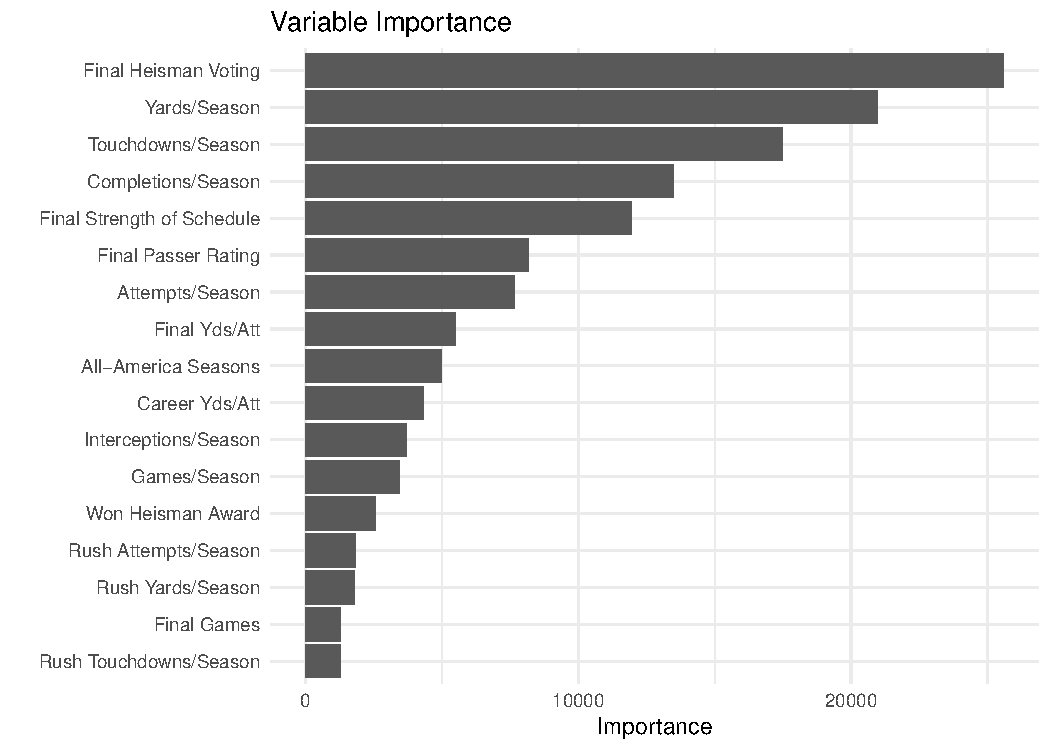
\includegraphics[width=0.75\linewidth]{../../figures/variable_importance.pdf}
    \caption{\textit{Variable importance plot for random forest trained to predict adjusted NFL QBR for college quarterbacks.}}
    \label{fig:importance}
\end{figure}

Figure \ref{fig:3d-plot} visualizes the prediction function learned by the random forest by plotting predicted adjusted QBR against career passing yards per season and final-season passer rating. These are two of the most important predictors in the model, and they have a relatively low correlation. The extreme outlier by passing yards per season is Bailey Zappe, who played only one FBS season at Western Kentucky in Conference USA and was selected by the New England Patriots in the fourth round of the 2022 NFL Draft. The predictions of the random forest model are conservative, with extremely few quarterbacks predicted to exceed an adjusted QBR of 40. This speaks to the large number of college quarterbacks who achieve zero QBR in the NFL and the difficulty of distinguishing between prospects based on college performance statistics alone.

\begin{figure}[H]
    \centering
    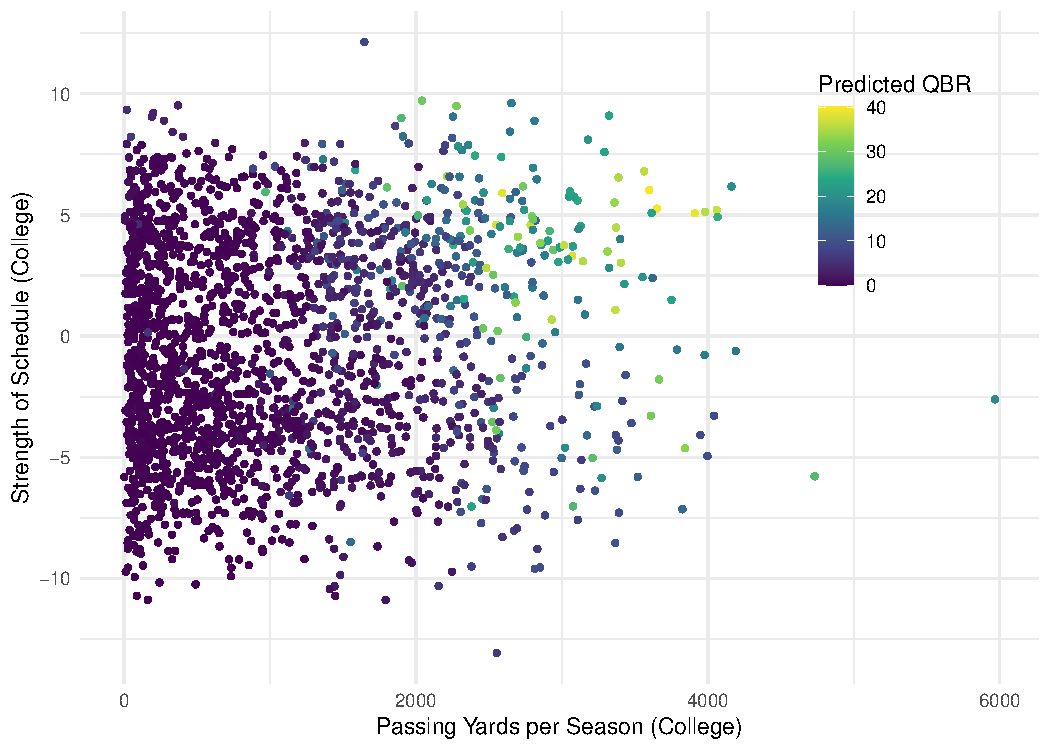
\includegraphics[width=0.75\linewidth]{../../figures/3d_plot.pdf}
    \caption{\textit{Predicted adjusted QBR plotted against average passing yards per season and final-season passer rating.}}
    \label{fig:3d-plot}
\end{figure}

Figure \ref{fig:predicted-vs-actuals} shows actual vs. predicted adjusted QBR for all quarterbacks in the dataset. Recall that 91\% of actual QBRs are zero, which the visualization does not make clear. The errors are very right-skewed, and this illustrates why no college quarterback exceed an adjusted QBR prediction of 50.

\begin{figure}[H]
  \centering
  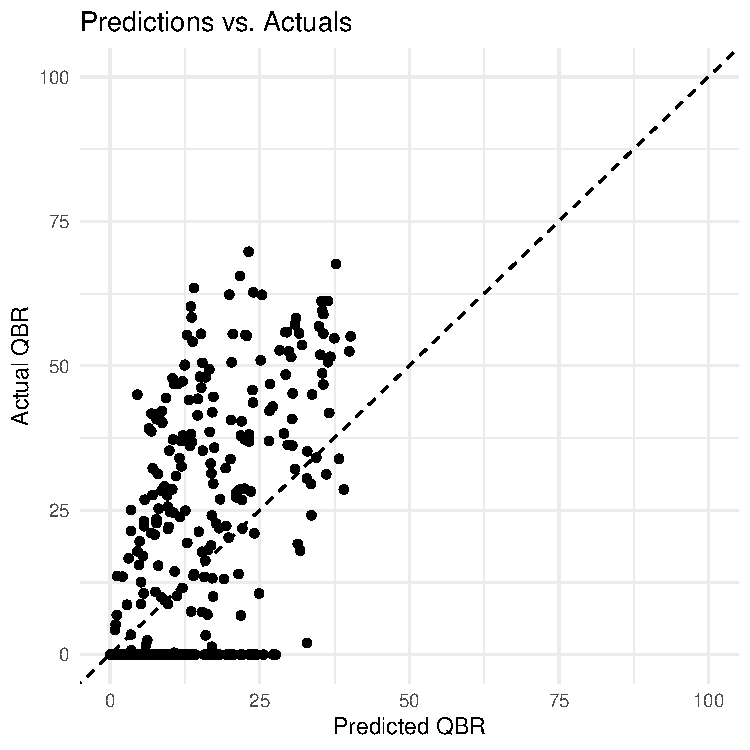
\includegraphics[width=0.5\linewidth]{../../figures/predicted_vs_actuals.pdf}
  \caption{\textit{Predicted (from random forest) and actual adjusted QBR for all quarterbacks in the dataset. The vats majority (91\%) of actual QBRs are zero, meaning that the points along the x-axis represent 91\% of the data.}}
  \label{fig:predicted-vs-actuals}
\end{figure}

\subsection{Case Study: 2025 NFL Draft}

Table \ref{tab:top-ten} shows the adjusted QBR predictions for the top 10 predicted quarterbacks in the 2025 draft. Cam Ward is predicted to have the highest adjusted QBR, which matches the common consensus that he was the best quarterback in this draft class and the fact he was taken first overall in the draft. Dillon Gabriel and Shedeur Sanders were projected to have the second and third highest adjusted QBRs, respectively. While Dillon Gabriel was not previously expected to be drafted as high as Shedeur Sanders, he had a very consistent college career and finished the highest out of any quarterback in Heisman voting in 2025. Jaxson Dart's draft stock increased substantially after the Scouting Combine and his pro day.

\begin{table}[H]
  \centering
  \begin{tabular}{l|r}
    Player & Predicted QBR\\
    \hline
    \begin{tabular}{l|r}
Player & Predicted QBR \\
% latex table generated in R 4.5.0 by xtable 1.8-4 package
% Mon Jul 28 14:59:35 2025
  \hline
Cameron Ward & 37.0 \\ 
  Dillon Gabriel & 34.6 \\ 
  Shedeur Sanders & 33.2 \\ 
  Jaxson Dart & 24.0 \\ 
  Quinn Ewers & 21.5 \\ 
  Kurtis Rourke & 19.9 \\ 
  Will Howard & 18.1 \\ 
  Will Rogers & 18.0 \\ 
  Max Brosmer & 17.6 \\ 
  Kyle McCord & 16.8 \\ 
\end{tabular}

  \end{tabular}
  \caption{\textit{Top ten career-average adjusted QBR predictions for quarterback prospects in the 2025 draft class. This includes only draft-eligible players who played at an NCAA Division I FBS school during the 2024 season.}}
  \label{tab:top-ten}
\end{table}

The predictions are interesting, but the focus of the present work is interpreting the predictions. Table \ref{tab:side-by-side-similarity} reports the ten most similar historical draft prospects for the top four quaterback prospects: Cam Ward, Shedeur Sanders, Jaxson Dart and Dillon Gabriel. Recall that the similarity scores reported in this table are interpretable as the weight of each historical prospect in the predictions in Table \ref{tab:top-ten}. Football fans will notice many household names among the comps for Ward, Sanders and Gabriel, but the comps for Dart are less impressive. Of note, the highest similarity score for any of these prospects is only 3.0\%. This is a helpful reminder that quarterback career outcomes are noisy, and the random forest model learns to spread out the weight across historical players, rather than concentrating a lot of weight in the single most similar player.

These four quarterback prospects illustrate the model's interpretability and its alignment with real-world outcomes. Sanders and Ward were both initially expected to go in the first round of the 2025 draft. Sanders' draft position unexpectedly slid, and he ended up being taken in the fifth round in the draft. However, this is likely a result of his refusal to participate in the NFL Scouting Combine, coupled with a reported bad attitude in his interviews, rather than his college performance \citep{mckenna_what_nodate}. In the end, Dart was the other quarterback taken in the first round of the draft.

\begin{table}[H]
  \resizebox{\textwidth}{!}{
    \begin{tabular}{lr|lr|lr|lr}
      \multicolumn{2}{c|}{\bf Cam Ward} &
        \multicolumn{2}{c|}{\bf Shedeur Sanders} &
        \multicolumn{2}{c|}{\bf Jaxson Dart} &
        \multicolumn{2}{c}{\bf Dillon Gabriel}\\
      Comp & Score & Comp & Score & Comp & Score & Comp & Score\\
      \hline
      \begin{tabular}{lr|lr|lr|lr}

      \multicolumn{2}{c|}{Cam Ward} &
      \multicolumn{2}{c|}{Dillon Gabriel} &
      \multicolumn{2}{c|}{Shedeur Sanders} &
      \multicolumn{2}{c}{Jaxson Dart}
    \\
Comp & Score & Comp & Score & Comp & Score & Comp & Score \\
% latex table generated in R 4.4.1 by xtable 1.8-4 package
% Tue Jul 29 12:31:28 2025
  \hline
Johnny Manziel & 2.3\% & Mason Rudolph & 2.0\% & Mason Rudolph & 1.9\% & Teddy Bridgewater & 1.9\% \\ 
  Marcus Mariota & 2.3\% & Dwayne Haskins & 1.9\% & Kenny Pickett & 1.9\% & Tajh Boyd & 1.6\% \\ 
  Baker Mayfield & 2.2\% & Kenny Pickett & 1.9\% & Philip Rivers & 1.9\% & Russell Wilson & 1.5\% \\ 
  Philip Rivers & 2.1\% & C.J. Stroud & 1.9\% & Ben Roethlisberger & 1.8\% & John Beck & 1.5\% \\ 
  Trevor Lawrence & 2.0\% & Andrew Luck & 1.9\% & Case Keenum & 1.8\% & Drake Maye & 1.4\% \\ 
  Matt Leinart & 2.0\% & Bo Nix & 1.9\% & Russell Wilson & 1.8\% & Zach Terrell & 1.4\% \\ 
  Russell Wilson & 2.0\% & Trevor Lawrence & 1.9\% & Trevone Boykin & 1.8\% & Kevin Hogan & 1.2\% \\ 
  Lamar Jackson & 1.9\% & Philip Rivers & 1.8\% & Kellen Moore & 1.7\% & Blake Bortles & 1.2\% \\ 
  Deshaun Watson & 1.9\% & Aaron Rodgers & 1.7\% & Andrew Luck & 1.7\% & Sam Howell & 1.2\% \\ 
  Case Keenum & 1.9\% & Bryce Young & 1.6\% & C.J. Stroud & 1.7\% & Patrick Mahomes & 1.1\% \\ 
\end{tabular}

    \end{tabular}
  }
  \caption{\textit{Top ten similarity scores for each of the top four quarterback prospects in the 2025 NFL draft. The similarity score is the contribution made by each historical prospect to the weighted average which constitutes the reference prospect's prediction in the random forest model.}}
  \label{tab:side-by-side-similarity}
\end{table}

It is worth noting that both Ward and Sanders started their college careers at teams that are not in the NCAA Division I FBS, as Ward played his first season at Incarnate Word and Sanders played his first two seasons at Jackson State. As a result, their college statistics used in the model do not include their statistics from these schools. We observe that Ward has the highest adjusted QBR prediction, which intuitively makes sense because he is widely regarded as the best quarterback in this year's draft class. Gabriel has a slightly higher QBR prediction than Sanders although Sanders was considered a better prospect. However, Gabriel finished higher than Sanders in Heisman voting, and Oregon had a much better record than Colorado, and Gabriel was ultimately taken before Sanders in the draft. Dart's relatively low prediction compared to the other three makes sense because he wasn't considered a top quarterback prospect until his performance in the NFL Combine, which this model does not take into consideration. He also performed well in his interviews with teams, which is not a quantifiable measure.

Figure \ref{fig:prospect-plots} provides a full breakdown of the random forest predictions based on the each prospect's similarity scores for all of the historical prospects in the training data. Each prospect's prediction is a weighted average of past prospect's outcomes, and the weighted histograms in Figure \ref{fig:prospect-plots} visualize that weighted mean. We observe that all four 2025 prospects have a large concentration of weight on training players with 0 QBR, a reminder that even top prospects have a danger of becoming busts. Ward has the highest concentration of comps between 55 and 65 QBR, which is why his prediction is the highest. On the opposite end of the spectrum, Dart has the highest concentration of training players near 0 QBR, explaining why his prediction was by far the lowest of the four prospects.

\begin{figure}[H]
    \centering
    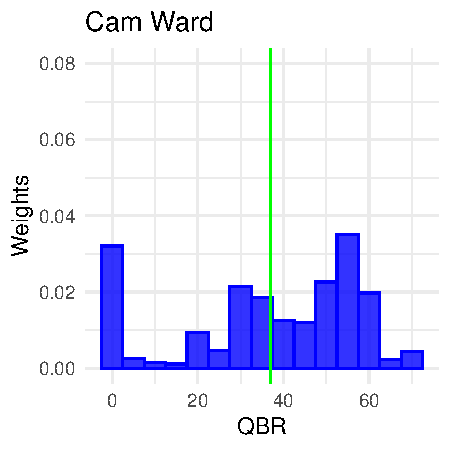
\includegraphics[width=0.24\linewidth]{../../figures/prospect_histogram_ward.pdf}
    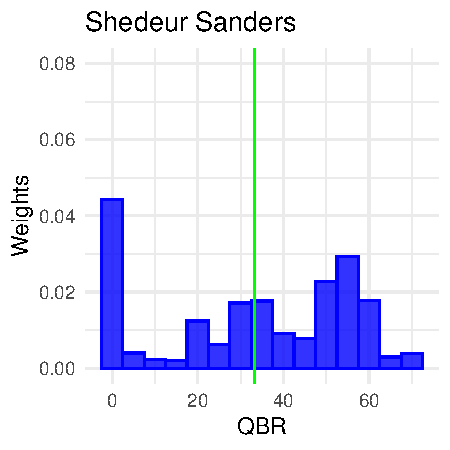
\includegraphics[width=0.24\linewidth]{../../figures/prospect_histogram_sanders.pdf}
    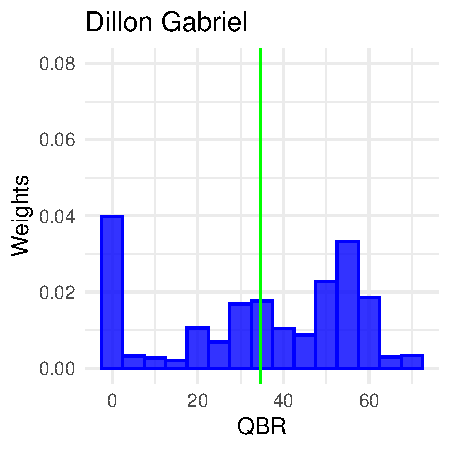
\includegraphics[width=0.24\linewidth]{../../figures/prospect_histogram_gabriel.pdf}
    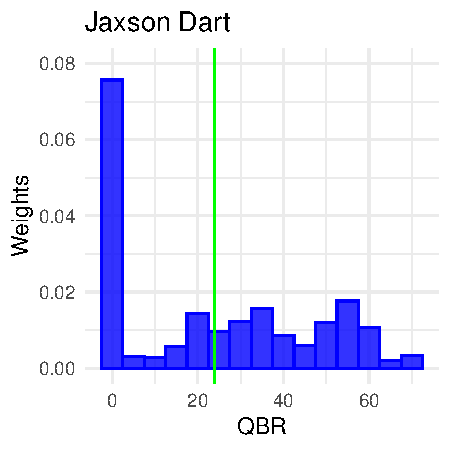
\includegraphics[width=0.24\linewidth]{../../figures/prospect_histogram_dart.pdf} \\
    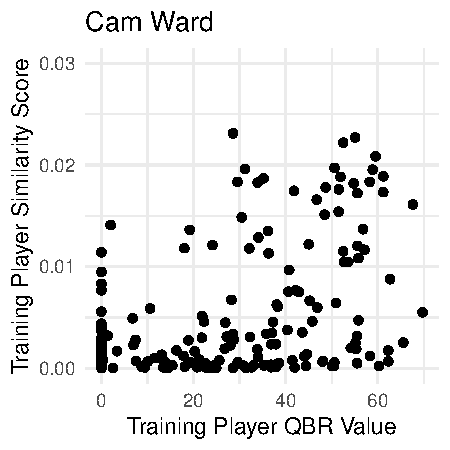
\includegraphics[width=0.24\linewidth]{../../figures/prospect_similarity_ward.pdf}
    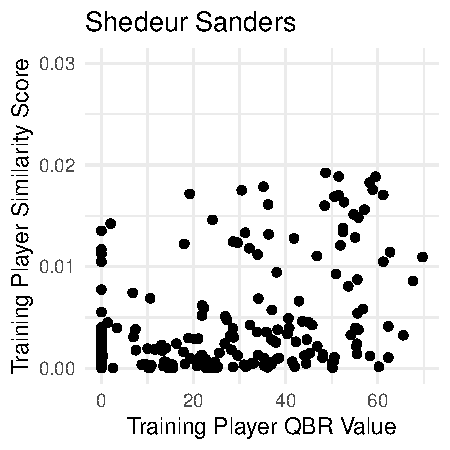
\includegraphics[width=0.24\linewidth]{../../figures/prospect_similarity_sanders.pdf}
    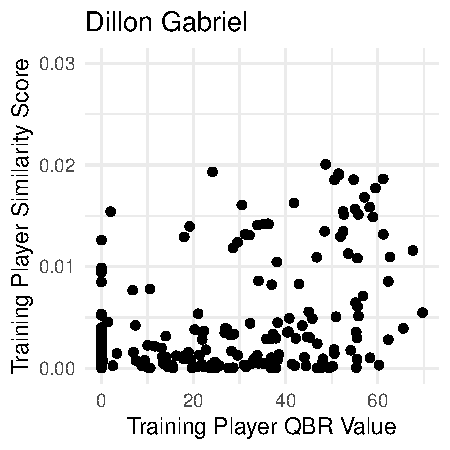
\includegraphics[width=0.24\linewidth]{../../figures/prospect_similarity_gabriel.pdf}
    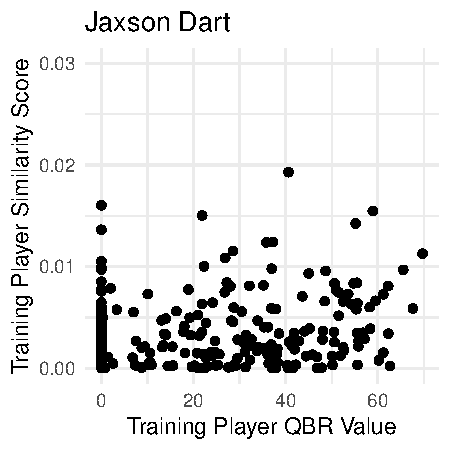
\includegraphics[width=0.24\linewidth]{../../figures/prospect_similarity_dart.pdf}
    \caption{\textit{Top: Histogram of training players' adjusted QBR values weighted by similarity to the reference prospect. The vertical green line annotates each prospect's predicted adjusted QBR, which matches the mean of the histograph distribution. Bottom: Scatter plot showing individual similarity scores and adjusted QBR for historical prospects.}}
    \label{fig:prospect-plots}
\end{figure}

\section{Software}
\label{sec:software}

\section{Discussion}
\label{sec:discussion}

We have demonstrated a methodology for producing similarity scores to help interpret the predictions of random forests. These similarity scores have the nice property that the random forest predictions are the weighted averages of outcomes in the training set, weighted according to these similarity scores. In addition to interpreting the random forest predictions, the methodology is helpful for identifying similar players based on the random forest as an adaptive $k$-NN algorithm, meaning that the neighborhoods are chosen in a meaningful way for predicting outcomes, which is not the case for a standard $k$-NN algorithm based on Euclidean distance. Our methodology is not limited to quarterbacks, to football, or even to sports, although the interpretation of predictions as a weighted average of historical comps fits well with the tradition of using comps in traditional scouting for sports.

In the application to the 2025 NFL draft, the random forest's predictions explain close to one third of the out-of-sample variance in adjusted QBR, which highlights some limitations of statistical forecasting when scouting draft prospects. The variable importance rankings show the college statistics that have a tendency to translate into better NFL performance. However, these two things also highlight the importance of non-quantifiable factors---such as attitude, coachability, off-the-field issues, adaptability, and leadership.

[INSERT PARAGRAPH ABOUT SOFTWARE]

[INSERT PARAGRAPH ABOUT FUTUR WORK EXTENDING TO OTHER TREE-BASED METHODS]

One key strength of this approach to comps is its objectivity. It enables teams to leverage historical data to make comps, without relying solely on scouting narratives or subjective analysis. While this approach should not replace traditional scouting, it can complement the existing strategies and provide additional information to front offices. 

\bibliography{../random-forest-comps}

\end{document}
